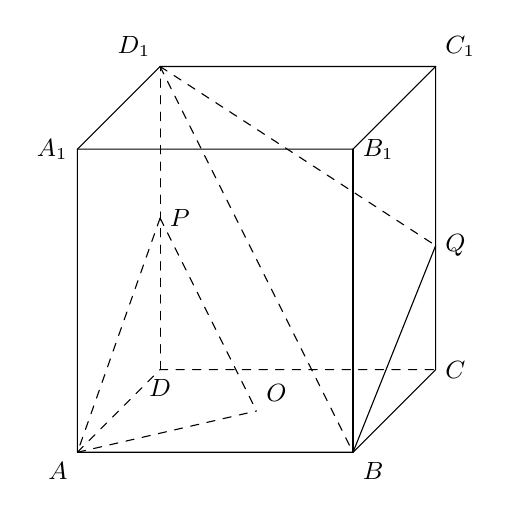
\begin{tikzpicture}[x=7mm,y=7mm,line cap=round,line join=round,every node/.style={font=\small}]
\coordinate (A)  at (0,0);
\coordinate (B)  at (5,0);
\coordinate (C)  at (6.5,1.5);
\coordinate (D)  at (1.5,1.5);
\coordinate (A1) at (0,5.5);
\coordinate (B1) at (5,5.5);
\coordinate (C1) at (6.5,7);
\coordinate (D1) at (1.5,7);
\coordinate (P)  at (1.5,4.25);
\coordinate (O)  at (3.25,.75);
\coordinate (Q)  at (6.5,3.75);

% Visible edges of the cube.
\draw (A)--(B)--(C)--(C1)--(D1)--(A1)--cycle;
\draw (A1)--(B1)--(C1);
\draw (B1)--(B);

% Hidden rear and lower edges.
\draw[dashed] (A)--(D)--(C);
\draw[dashed] (D)--(D1);

% Auxiliary segments in the two indicated planes.
\draw[dashed] (D1)--(B);
\draw[dashed] (D1)--(Q);
\draw[dashed] (P)--(A);
\draw[dashed] (P)--(O);
\draw[dashed] (A)--(O);
\draw (B)--(Q);

\node[below left]  at (A)  {$A$};
\node[below right] at (B)  {$B$};
\node[right]       at (C)  {$C$};
\node[below]       at (D)  {$D$};
\node[left]        at (A1) {$A_1$};
\node[right]       at (B1) {$B_1$};
\node[above right] at (C1) {$C_1$};
\node[above left]  at (D1) {$D_1$};
\node[right]       at (P)  {$P$};
\node[above right] at (O)  {$O$};
\node[right]       at (Q)  {$Q$};
\end{tikzpicture}
